\chapter{Arhitektura i dizajn sustava}
		
		%\textbf{\textit{dio 1. revizije}}\\

		%\textit{ Potrebno je opisati stil arhitekture te identificirati: podsustave, preslikavanje na radnu platformu, spremišta podataka, mrežne protokole, globalni upravljački tok i sklopovsko-programske zahtjeve. Po točkama razraditi i popratiti odgovarajućim skicama:}
	%\begin{itemize}
		%\item 	\textit{izbor arhitekture temeljem principa oblikovanja pokazanih na predavanjima (objasniti zašto ste baš odabrali takvu arhitekturu)}
		%\item 	\textit{organizaciju sustava s najviše razine apstrakcije (npr. klijent-poslužitelj, baza podataka, datotečni sustav, grafičko sučelje)}
		%\item 	\textit{organizaciju aplikacije (npr. slojevi frontend i backend, MVC arhitektura) }		
	%\end{itemize}

	Stil arhitekture koji smo odabrali je arhitektura zasnovana na događajima gdje se događaji javno objavljuju te se pozivaju registrirane procedure, dok komponente koje objavljuju događaj nemaju informaciju koje će sve komponente reagirati i kako. Za razliku od objektno usmjerenog stila, komponente se ne pozivaju eksplicitno, već generiraju signale, tj. događaje. Ova arhitektura je odabrana jer je najefikasnija za obradu korisničkih zahtjeva, laka je za održavanje i reciklabilna za potrebe budućih projekata ili nadogradnje ovog. Što se tiče spremišta podataka, svi podaci će biti spremani te dohvaćani iz univerzalne baze podataka. Mrežni protokoli koji će se pozivati tokom komunikacije klijenta s poslužiteljem su: TCP, IP, HTTP. 
Sustav je organiziran na sljedeći način: 
\begin{figure}[H]
			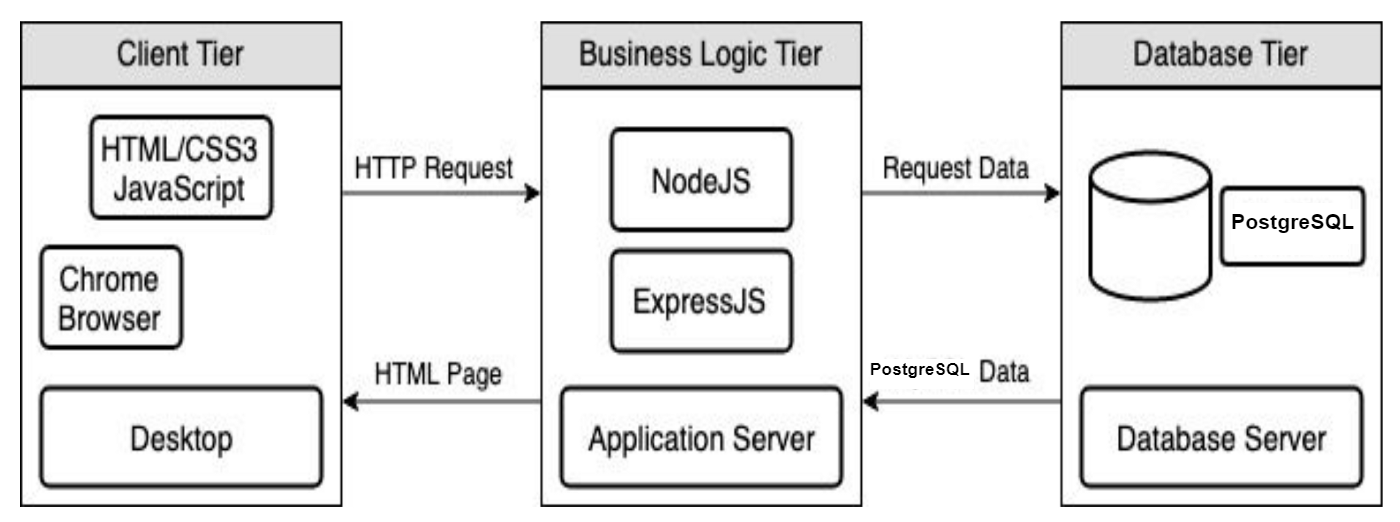
\includegraphics[width=\textwidth]{slike/arhitekturaSkica.png} %veličina u odnosu na širinu linije
			\caption{grafički prikaz arhitekture}
			\label{fig:arhitektura} %label mora biti drugaciji za svaku sliku
			\end{figure}
Korisnik putem odabranog web preglednika šalje HTTP zahtjev za web aplikacijom i njenim komponentama zadanom web poslužitelju. Aplikacija komunicira s bazom podataka u kojoj su sadržani svi podatci i iz nje izvlači sve potrebne podatke za klijentov zahtjev. Poslužitelj, kada aplikacija dohvati sve potrebne podatke, odgovara na klijentov zahtjev sa statusom 200 OK (ako je sve u redu) i šalje mu HTML dokument koji se prikazuje u zadanom web pregledniku.
Programski jezik koji smo koristili za izradu web aplikacije je Java za backend te Javascript za frontend dio.
Arhitektura sustava se temelji na MVC konceptu, stilističkoj varijaciji arhitekture zasnovanoj na događajima. Odabrali smo taj koncept jer odvaja korisničko sučelje od ostatka sustava, što čini razvoj i nadogradnju komponenata jednostavnijima. Sastoji se od modela, pogleda i upravitelja.
		
\begin{itemize}
\item Model – dojavljuje sebi pridruženim pogledima i upravitelju kada je došlo do promjene u njegovom stanju. Ove dojave omogućuju pogledu da prikaže obnovljeno stanje modela, a upravitelju promjenu dostupnog skupa naredbi
\item View (Pogled) - od modela dobija informacije koje su mu potrebne za prikaz korisniku
\item Controller (Upravitelj)  – šalje naloge modelu koji ažurira svoje stanje i naredbe pogledima kojima mijenja prikaz modela
\end{itemize}
		

				
		\section{Baza podataka}
			
			%\textbf{\textit{dio 1. revizije}}\\
			
		%\textit{Potrebno je opisati koju vrstu i implementaciju baze podataka ste odabrali, glavne komponente od kojih se sastoji i slično.}
		Za potrebe našeg sustava koristit ćemo relacijsku bazu podataka koja svojom strukturom nam olakšava da zorno modeliramo stvarni svijet. Baza podataka se sastoji od tablica definiranih imenom i  atributima. Zadaća baze podataka je brza i jednostavna pohrana, izmjena i dohvat podataka za daljnju obradu. Baza podataka sastoji se od ovih entiteta: 
		\begin{itemize}
		\item Korisnik
\item Proizvod
\item Oznake
\item Komentar
\item Pretinac
\item Privatnost
\item Obavijest
\item ProizvodTrgovina
\item PromjenaCijenaKorisnik
\item PromjenaCijenaTrgovina
\item Trgovina
\item session
		\end{itemize}

		
			\subsection{Opis tablica}
			

				%\textit{Svaku tablicu je potrebno opisati po zadanom predlošku. Lijevo se nalazi točno ime varijable u bazi podataka, u sredini se nalazi tip podataka, a desno se nalazi opis varijable. Svjetlozelenom bojom označite primarni ključ. Svjetlo plavom označite strani ključ}
				
				
				%\begin{longtblr}[
				%	label=none,
				%	entry=none
				%	]{
				%		width = \textwidth,
				%		colspec={|X[6,l]|X[6, l]|X[20, l]|}, 
				%		rowhead = 1,
				%	} %definicija širine tablice, širine stupaca, poravnanje i broja redaka naslova tablice
				%	\hline \multicolumn{3}{|c|}{\textbf{korisnik - ime tablice}}	 \\ \hline[3pt]
				%	\SetCell{LightGreen}IDKorisnik & INT	&  	Lorem ipsum dolor sit amet, consectetur adipiscing elit, sed do eiusmod  	\\ \hline
				%	korisnickoIme	& VARCHAR &   	\\ \hline 
				%	email & VARCHAR &   \\ \hline 
				%	ime & VARCHAR	&  		\\ \hline 
				%	\SetCell{LightBlue} primjer	& VARCHAR &   	\\ \hline 
				%\end{longtblr}
				
Entitet \textbf{Korisnik} sadržava sve važne informacije o registriranim korisnicima aplikacije.
Sadrži atribute: ID, Ime, Prezime, Email, Nadimak, Lozinka, RazinaPristupa i ZabranjenPristup.
Ovaj entitet u vezi je One-to-Many s Oznake preko KorisnikID, u vezi je Many-to-Many s Komentar preko KorisnikID, u vezi je Many-to-Many s Pretinac preko KorisnikID, u vezi je One-to-One s Privatnost preko KorisnikID i u vezi je Many-to-Many s PromjenaCijenaKorisnik preko KorisnikID.
				\begin{longtblr}[
label=none,
entry=none
]{
width = \textwidth,
colspec={|X[6,l]|X[6, l]|X[20, l]|}, 
rowhead = 1,
} %definicija širine tablice, širine stupaca, poravnanje i broja redaka naslova tablice
\hline \multicolumn{3}{|c|}{\textbf{Korisnik}}	 \\ \hline[3pt]
\SetCell{LightGreen}ID & INT	&  	Unikatni identifikator svakog prijavljenog korisnika  	\\ \hline
Ime	& VARCHAR &  Ime korisnika 	\\ \hline 
Prezime	& VARCHAR &  Prezime korisnika 	\\ \hline 
Email & VARCHAR &  Email korisnika \\ \hline 
Nadimak & VARCHAR	&  Unikatni nadimak korisnika	\\ \hline 
Lozinka & VARCHAR	&  Korisnikova lozinka za pristup računu	\\ \hline 
RazinaPristupa & SMALLINT	&  Ako je 0 onda je registrirani korisnik, ako je 1 onda je trgovina i ako je 2 onda je administrator	\\ \hline 
ZabranjenPristup & BOOLEAN & Ako je true onda je administrator zabranio pristup ovom profilu \\ \hline
\end{longtblr}


Entitet \textbf{Trgovina} sadržava informacije vezane za određenu trgovinu.
Sadrži atribute: ID i Naziv.
Ovaj entitet u vezi je Many-to-Many s entitetom PromjenaCijenaTrgovina preko atributa TrgovinaID, u vezi je Many-to-Many PromjenaCijenaKorisnik preko atributa TrgovinaID, u vezi je Many-to-Many ProizvodTrgovina preko atributa TrgovinaID i u vezi je Many-to-One s entitetom Komentar preko atributa TrgovinaID.
\begin{longtblr}[
label=none,
entry=none
]{
width = \textwidth,
colspec={|X[6,l]|X[6, l]|X[20, l]|}, 
rowhead = 1,
} %definicija širine tablice, širine stupaca, poravnanje i broja redaka naslova tablice
\hline \multicolumn{3}{|c|}{\textbf{Trgovina}}	 \\ \hline[3pt]
\SetCell{LightGreen}ID & INT	&  	Unikatni identifikator svake trgovine  	\\ \hline
Naziv	& VARCHAR &  Naziv trgovine 	\\ \hline 
\end{longtblr}

Entitet \textbf{Proizvod} sadržava osnovne informacije o proizvodima.
Sadrži atribute: Barkod i Naziv.
Ovaj entitet u vezi je Many-to-Many s entitetom Oznake preko atributa Barkod, u vezi je One-to-Many s ProizvodTrgovina preko atributa Barkod, u vezi je One-to-Many s PromjenaCijenaKorisnik preko atributa Barkod i u vezi je  One-to-Many s PromjenaCijenaTrgovina preko atributa Barkod.
\begin{longtblr}[
label=none,
entry=none
]{
width = \textwidth,
colspec={|X[6,l]|X[6, l]|X[20, l]|}, 
rowhead = 1,
} %definicija širine tablice, širine stupaca, poravnanje i broja redaka naslova tablice
\hline \multicolumn{3}{|c|}{\textbf{Proizvod}}	 \\ \hline[3pt]
\SetCell{LightGreen}Barkod & VARCHAR	&  	Unikatni identifikator proizvoda  	\\ \hline
Naziv & VARCHAR	&  Naziv proizvoda		\\ \hline 
\end{longtblr}

Entitet \textbf{Komentar} sadržava zapise o komentarima napisanim od administratora za određenu trgovinu.
Sadrži atribute: KorisnikID, TrgovinaID i OpisKomentara.
Ovaj entitet u vezi je One-to-Many s entitetom Trgovina preko atributa TrgovinaID i u vezi 
Many-to-Many s Korisnik preko KorisnikID.
\begin{longtblr}[
label=none,
entry=none
]{
width = \textwidth,
colspec={|X[6,l]|X[6, l]|X[20, l]|}, 
rowhead = 1,
} %definicija širine tablice, širine stupaca, poravnanje i broja redaka naslova tablice
\hline \multicolumn{3}{|c|}{\textbf{Komentar}}	 \\ \hline[3pt]
\SetCell{LightBlue} KorisnikID	& INT &   Identifikator korisnika koji je napisao komentar	\\ \hline 
\SetCell{LightBlue} TrgovinaID	& INT &   Identifikator trgovine kod koje je komentirani proizvod	\\ \hline 
OpisKomentara	& VARCHAR &  Upisani komentar		\\ \hline 
\end{longtblr}


Entitet \textbf{Obavijest} sadržava informacije vezane za određenu obavijest.
Sadrži atribute: ID, DatumVrijeme, Opis i Procitano.
Ovaj entitet u vezi je Many-to-One s entitetom Pretinac preko atributa ObavijestID.
\begin{longtblr}[
label=none,
entry=none
]{
width = \textwidth,
colspec={|X[6,l]|X[6, l]|X[20, l]|}, 
rowhead = 1,
} %definicija širine tablice, širine stupaca, poravnanje i broja redaka naslova tablice
\hline \multicolumn{3}{|c|}{\textbf{Obavijest}}	 \\ \hline[3pt]
\SetCell{LightGreen}ID & INT	&  	Unikatni identifikator obavijesti  	\\ \hline
DatumVrijeme & TIMESTAMP & Vrijeme kada je dostavljena obavijest \\ \hline
Opis	& VARCHAR &  Opis obavijesti 	\\ \hline 
Procitano & BOOLEAN & Ako je True onda je korisnik pročitao obavijest \\ \hline
\end{longtblr}


Entitet \textbf{Oznake} sadržava zapise o proizvodima s oznakama stavljenim od korisnika.
Sadrži atribute: Barkod, KorisnikID i Oznaka.
Ovaj entitet u vezi je Many-to-Many s entitetom Proizvod preko atributa Barkod i u vezi 
Many-to-One s Korisnik preko KorisnikID.
\begin{longtblr}[
label=none,
entry=none
]{
width = \textwidth,
colspec={|X[6,l]|X[6, l]|X[20, l]|}, 
rowhead = 1,
} %definicija širine tablice, širine stupaca, poravnanje i broja redaka naslova tablice
\hline \multicolumn{3}{|c|}{\textbf{Oznake}}	 \\ \hline[3pt]
\SetCell{LightBlue} Barkod	& VARCHAR &   Identifikator proizvoda pod kojim je oznaka	\\ \hline 
\SetCell{LightBlue} KorisnikID	& INT &   Identifikator korisnika koji je napisao oznaku	\\ \hline 
Oznake	& VARCHAR &  Naziv oznake		\\ \hline 
\end{longtblr}


Entitet \textbf{Pretinac} sadržava zapise o obavijestima kod korisnika.
Sadrži atribute: KorisnikID i ObavijestID.
Ovaj entitet u vezi je One-to-Many s entitetom Obavijest preko atributa ObavijestID i u vezi 
Many-to-Many s Korisnik preko KorisnikID.
\begin{longtblr}[
label=none,
entry=none
]{
width = \textwidth,
colspec={|X[6,l]|X[6, l]|X[20, l]|}, 
rowhead = 1,
} %definicija širine tablice, širine stupaca, poravnanje i broja redaka naslova tablice
\hline \multicolumn{3}{|c|}{\textbf{Pretinac}}	 \\ \hline[3pt]
\SetCell{LightBlue} KorisnikID	& INT &   Identifikator korisnika koji je dobio obavijest	\\ \hline 
\SetCell{LightBlue} ObavijestID	& INT &   Identifikator obavijesti \\ \hline 
\end{longtblr}


Entitet \textbf{Privatnost} sadržava zapise o kojim informacijama se prikazuju na profilu korisnika.
Sadrži atribute: KorisnikID, Ime,  Prezime, Email i Nadimak.
Ovaj entitet je u vezi One-to-One s Korisnik preko KorisnikID.
\begin{longtblr}[
label=none,
entry=none
]{
width = \textwidth,
colspec={|X[6,l]|X[6, l]|X[20, l]|}, 
rowhead = 1,
} %definicija širine tablice, širine stupaca, poravnanje i broja redaka naslova tablice
\hline \multicolumn{3}{|c|}{\textbf{Privatnost}}	 \\ \hline[3pt]
\SetCell{LightBlue}KorisnikID & INT	&  	Identifikator korisnika 	\\ \hline
Ime	& BOOLEAN &  Ako je true onda se ime prikazuje na profilu, ako je false onda se ne prikazuje	\\ \hline 
Prezime	& BOOLEAN &  Ako je true onda se prezime prikazuje na profilu, ako je false onda se ne prikazuje \\ \hline 
Email	& BOOLEAN &  Ako je true onda se email prikazuje na profilu, ako je false onda se ne prikazuje \\ \hline 
Nadimak	& BOOLEAN &  Ako je true onda se nadimak prikazuje na profilu, ako je false onda se ne prikazuje \\ \hline 
\end{longtblr}



Entitet \textbf{ProizvodTrgovina} sadržava zapise o proizvodima u trgovinama.
Sadrži atribute: Barkod, TrgovinaID i Cijena.
Ovaj entitet u vezi je Many-to-Many s entitetom Trgovina preko atributa TrgovinaID i u vezi 
Many-to-One s Proizvod preko Barkod.
\begin{longtblr}[
label=none,
entry=none
]{
width = \textwidth,
colspec={|X[6,l]|X[6, l]|X[20, l]|}, 
rowhead = 1,
} %definicija širine tablice, širine stupaca, poravnanje i broja redaka naslova tablice
\hline \multicolumn{3}{|c|}{\textbf{ProizvodTrgovina}}	 \\ \hline[3pt]
\SetCell{LightBlue} Barkod	& VARCHAR &   Identifikator proizvoda	\\ \hline 
\SetCell{LightBlue} TrgovinaID	& INT &   Identifikator trgovine u kojoj je proizvod	\\ \hline 
Cijena	& MONEY &  Cijena proizvoda u određenoj trgovini		\\ \hline 
\end{longtblr}



Entitet \textbf{PromjenaCijeneKorisnik} sadržava zapise o promjenama cijena koje je upisao korisnik.
Sadrži atribute: KorisnikID, Barkod, TrgovinaID, DatumVrijeme, NovaCijena, Slika i Status.
Ovaj entitet u vezi je Many-to-Many s entitetom Korisnik preko atributa KorisnikID, u vezi 
Many-to-One s Proizvod preko Barkod i u vezi  Many-to-Many s Trgovina preko atributa TrgovinaID.
\begin{longtblr}[
label=none,
entry=none
]{
width = \textwidth,
colspec={|X[6,l]|X[6, l]|X[20, l]|}, 
rowhead = 1,
} %definicija širine tablice, širine stupaca, poravnanje i broja redaka naslova tablice
\hline \multicolumn{3}{|c|}{\textbf{PromjenaCijeneKorisnik}}	 \\ \hline[3pt]
\SetCell{LightBlue} Barkod	& VARCHAR &   Identifikator proizvoda	\\ \hline 
\SetCell{LightBlue} KorisnikID	& INT &   Identifikator korisnika koji je upisao promjenu cijene	\\ \hline 
\SetCell{LightBlue} TrgovinaID	& INT &   Identifikator trgovine gdje je pogrešna cijena	\\ \hline 
\SetCell{LightGreen} DatumVrijeme & TIMESTAMP & Vrijeme unosa nove cijene \\ \hline
NovaCijena	& MONEY &  Nova cijena proizvoda u određenoj trgovini		\\ \hline 
Slika & VARBIT & Slika kao dokaz nove cijene  \\ \hline
Status & VARCHAR & Kakav je status promjene cijene \\ \hline
\end{longtblr}


Entitet \textbf{PromjenaCijeneTrgovina} sadržava zapise o promjenama cijena koje je upisala trgovina.
Sadrži atribute: Barkod, TrgovinaID, DatumVrijeme, NovaCijena, Slika i Status.
Ovaj entitet u vezi je Many-to-Many s entitetom Trgovina preko atributa TrgovinaID i u vezi 
Many-to-One s Proizvod preko Barkod.
\begin{longtblr}[
label=none,
entry=none
]{
width = \textwidth,
colspec={|X[6,l]|X[6, l]|X[20, l]|}, 
rowhead = 1,
} %definicija širine tablice, širine stupaca, poravnanje i broja redaka naslova tablice
\hline \multicolumn{3}{|c|}{\textbf{PromjenaCijeneTrgovina}}	 \\ \hline[3pt]
\SetCell{LightBlue} Barkod	& VARCHAR &   Identifikator proizvoda	\\ \hline 
\SetCell{LightBlue} TrgovinaID	& INT &   Identifikator trgovine gdje je promjena cijene	\\ \hline 
\SetCell{LightGreen} DatumVrijeme & TIMESTAMP & Vrijeme unosa nove cijene \\ \hline
NovaCijena	& MONEY &  Nova cijena proizvoda u određenoj trgovini		\\ \hline 
\end{longtblr}

Entitet \textbf{session} sadržava zapise o sjednicama.
Sadrži atribute: sid, sess i expire.
\begin{longtblr}[
label=none,
entry=none
]{
width = \textwidth,
colspec={|X[6,l]|X[6, l]|X[20, l]|}, 
rowhead = 1,
} %definicija širine tablice, širine stupaca, poravnanje i broja redaka naslova tablice
\hline \multicolumn{3}{|c|}{\textbf{session}}	 \\ \hline[3pt]
\SetCell{LightGreen} sid	& VARCHAR &   Identifikator sjednice	\\ \hline 
sess & JSON & Json zapis sjednice \\ \hline
expire	& TIMESTAMP &  Datum i vrijeme isteka sjednice		\\ \hline 
\end{longtblr}
			
			\subsection{Dijagram baze podataka}
				%\textit{ U ovom potpoglavlju potrebno je umetnuti dijagram baze podataka. Primarni i strani ključevi moraju biti označeni, a tablice povezane. Bazu podataka je potrebno normalizirati. Podsjetite se kolegija "Baze podataka".}
				\begin{figure}[H]
			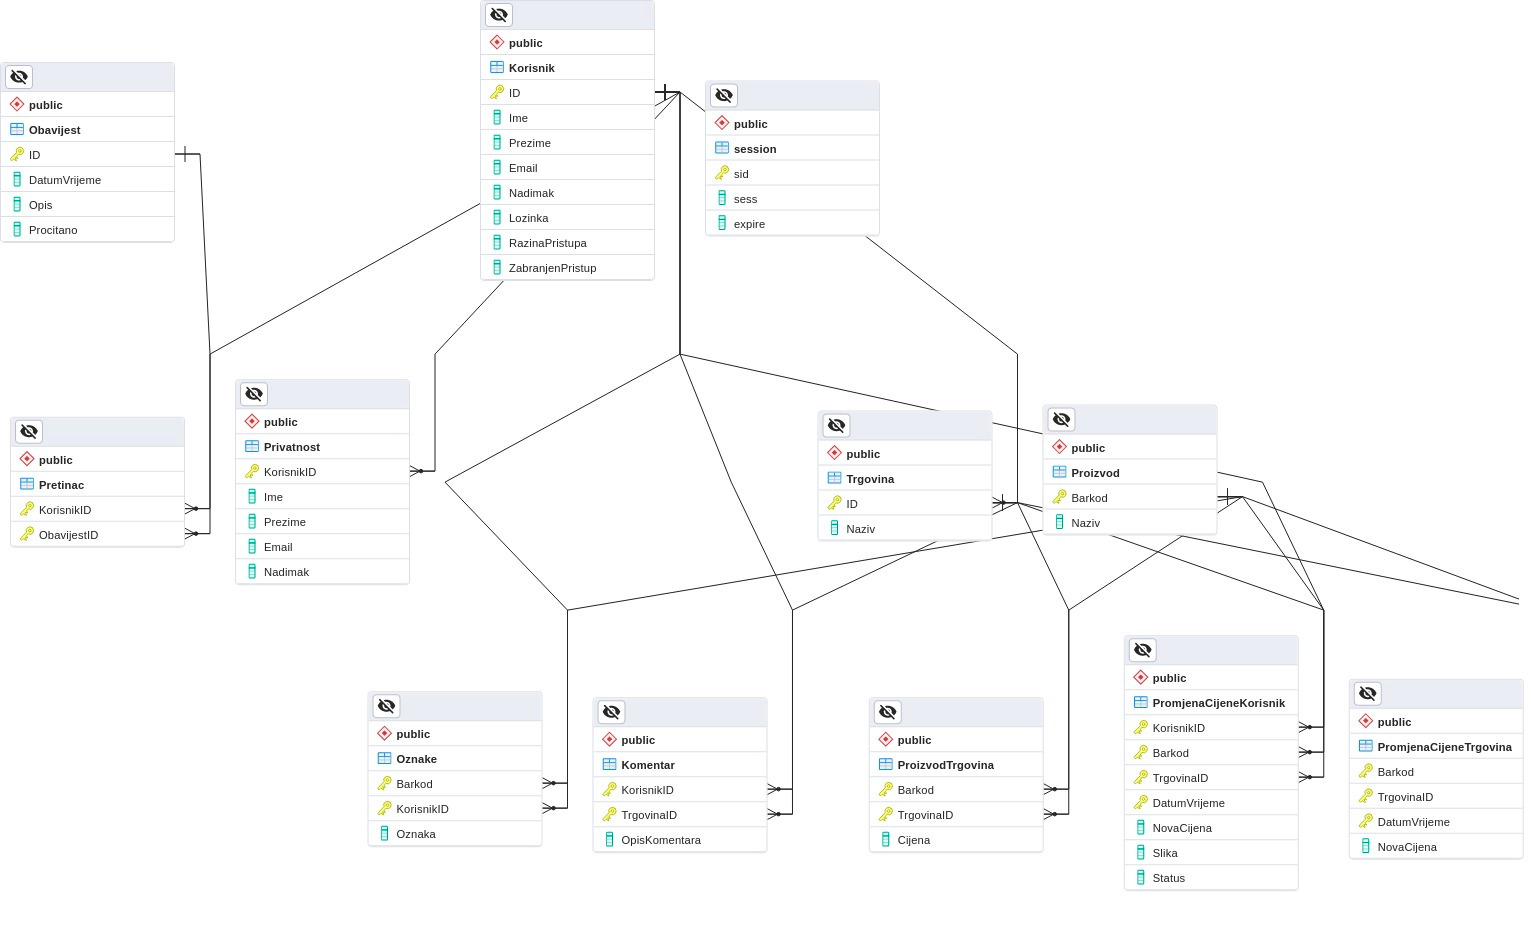
\includegraphics[width=\textwidth]{slike/ERDijagramBaza.JPEG} %veličina u odnosu na širinu linije
			\caption{E-R Dijagram baze podataka}
			\label{fig:ERDijagramBaza} %label mora biti drugaciji za svaku sliku
			\end{figure}
			
			\eject
			
			
		\section{Dijagram razreda}
		
			%\textit{Potrebno je priložiti dijagram razreda s pripadajućim opisom. Zbog preglednosti je moguće dijagram razlomiti na više njih, ali moraju biti grupirani prema sličnim razinama apstrakcije i srodnim funkcionalnostima.}\\
			\textbf{UserModel} služi za spremanje podataka o korisniku te za autentifikaciju i autorizaciju korisnika. 
			\textbf{UserModel} generalizira \textbf{Admin} i \textbf{StoreModel}.
			 
			\textbf{PrivacyModel} pohranjuje podatke o tome koji će podaci o korisniku biti javni, a koji privatni.
			  
			\textbf{Admin} sadrži metode koje može izvršiti isključivo korisnik s admin pravom pristupa(odobravanje promjena cijena, zabrana pristupa drugim korisnicima...) 
			
			\textbf{StoreModel} modelira trgovinu. 
			
			\textbf{ProductModel} modelira proizvod. Proizvod je jednoznačno određen barkodom kako bi više trgovina moglo imati isti proizvod u ponudi. 
			
			\textbf{PriceChangeLog} služi za opisivanje promjena cijena proizvoda u nekoj trgovini u nekom vremenskom razdoblju. 
			
			\textbf{PriceChangeRequestModel} modelira zahtjev za promjenom cijene koje šalje korisnik za proizvod u nekoj trgovini u kojoj se stvarna cijena razlikuje od cijene navedene u aplikaciji.  
			
			\textbf{NotificationModel} modelira obavijesti koje admin može slati korisniku ili trgovini.
Klase iz data access paketa sadržavaju isključivo statičke metode koje služe za komunikaciju s bazom podataka.

\begin{figure}[H]
			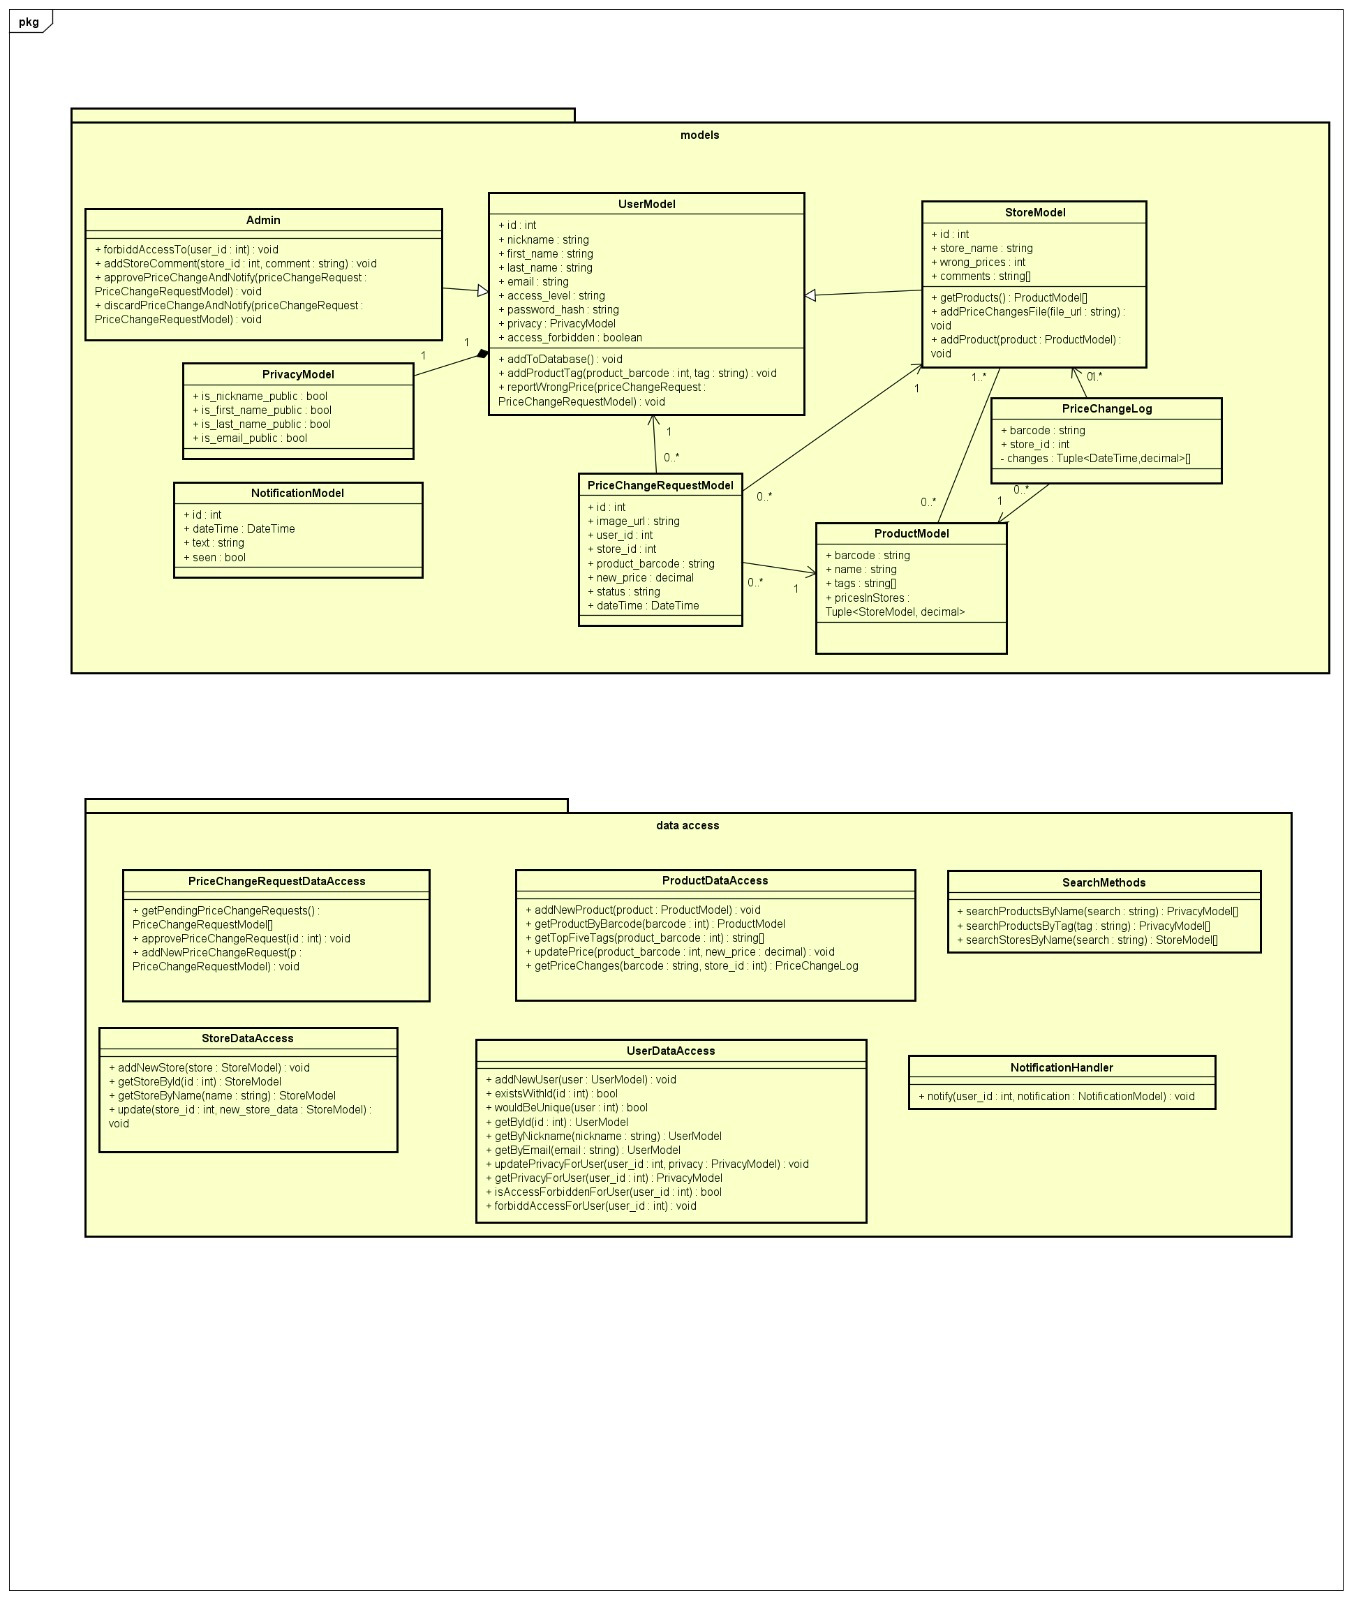
\includegraphics[width=\textwidth]{slike/dijagramRazreda.png} %veličina u odnosu na širinu linije
			\caption{dijagram razreda}
			\label{fig:dijagramRazreda} %label mora biti drugaciji za svaku sliku
			\end{figure}
			
			%\textbf{\textit{dio 1. revizije}}\\
			
			%\textit{Prilikom prve predaje projekta, potrebno je priložiti potpuno razrađen dijagram razreda vezan uz \textbf{generičku funkcionalnost} sustava. Ostale funkcionalnosti trebaju biti idejno razrađene u dijagramu sa sljedećim komponentama: nazivi razreda, nazivi metoda i vrste pristupa metodama (npr. javni, zaštićeni), nazivi atributa razreda, veze i odnosi između razreda.}\\
			
			%\textbf{\textit{dio 2. revizije}}\\			
			
			%\textit{Prilikom druge predaje projekta dijagram razreda i opisi moraju odgovarati stvarnom stanju implementacije}
			
			
			
			\eject
		
		%\section{Dijagram stanja}
			
			
			%\textbf{\textit{dio 2. revizije}}\\
			
			%\textit{Potrebno je priložiti dijagram stanja i opisati ga. Dovoljan je jedan dijagram stanja koji prikazuje \textbf{značajan dio funkcionalnosti} sustava. Na primjer, stanja korisničkog sučelja i tijek korištenja neke ključne funkcionalnosti jesu značajan dio sustava, a registracija i prijava nisu. }
			
			
			%\eject 
		
		%\section{Dijagram aktivnosti}
			
			%\textbf{\textit{dio 2. revizije}}\\
			
			% \textit{Potrebno je priložiti dijagram aktivnosti s pripadajućim opisom. Dijagram aktivnosti treba prikazivati značajan dio sustava.}
			
		%	\eject
		%\section{Dijagram komponenti}
		
			%\textbf{\textit{dio 2. revizije}}\\
		
			% \textit{Potrebno je priložiti dijagram komponenti s pripadajućim opisom. Dijagram komponenti treba prikazivati strukturu cijele aplikacije.}